\documentclass[12pt,a4paper]{article}

% ===== 中文支持 =====
\usepackage[UTF8]{ctex}

% ===== 页面设置 =====
\usepackage[top=2.5cm, bottom=2.5cm, left=2.5cm, right=2.5cm]{geometry}
\usepackage{setspace}
\onehalfspacing

% ===== 常用宏包 =====
\usepackage{graphicx}
\usepackage{booktabs}
\usepackage{longtable}
\usepackage{array}
\usepackage{float}
\usepackage{caption}
\usepackage{subcaption}
\usepackage{amsmath}
\usepackage{hyperref}
\usepackage{xcolor}
\usepackage{listings}
% enumitem 未安装，使用默认 enumerate 样式
\usepackage{tikz}
\usetikzlibrary{shapes.geometric, arrows.meta, positioning, fit, calc}

% ===== 代码样式 =====
\lstset{
    language=Python,
    basicstyle=\small\ttfamily,
    keywordstyle=\color{blue}\bfseries,
    commentstyle=\color{gray},
    stringstyle=\color{red!70!black},
    numbers=left,
    numberstyle=\tiny\color{gray},
    numbersep=8pt,
    frame=single,
    framesep=5pt,
    breaklines=true,
    breakatwhitespace=true,
    showstringspaces=false,
    tabsize=4,
    captionpos=b,
    xleftmargin=15pt,
    xrightmargin=5pt,
    aboveskip=10pt,
    belowskip=10pt,
}

% ===== 超链接样式 =====
\hypersetup{
    colorlinks=true,
    linkcolor=blue!70!black,
    citecolor=blue!70!black,
    urlcolor=blue!70!black,
}

% ===== 页眉页脚 =====
\usepackage{fancyhdr}
\pagestyle{fancy}
\fancyhf{}
\fancyhead[L]{\small BITMZ043 云计算与大数据分析}
\fancyhead[R]{\small 基于 Spark 的实时数据分析}
\fancyfoot[C]{\thepage}
\renewcommand{\headrulewidth}{0.4pt}

% ===== 标题信息 =====
\title{
    \vspace{-1cm}
    {\LARGE\textbf{基于 Spark Structured Streaming 的\\实时热门统计系统}} \\[0.5cm]
    {\large BITMZ043 云计算与大数据分析 \quad 课程实践报告} \\[0.3cm]
    {\normalsize 方向 C：基于 Spark 的实时数据分析}
}
\author{
    \textbf{姓名}：赵英杰 \quad \textbf{学号}：D23090600756 \\[0.2cm]
    \textbf{姓名}：韦多展 \quad \textbf{学号}：D23090600792
}
\date{\today}

% ===== 正文开始 =====
\begin{document}

\maketitle
\thispagestyle{fancy}

% ===== 摘要 =====
\begin{abstract}
本项目基于 Apache Spark Structured Streaming 框架，结合 Apache Kafka 消息队列，构建了一个面向电商场景的实时热门统计系统。系统实现了实时热门商品 Top-N 排行和实时热搜词统计两大核心功能，采用滑动窗口聚合与 Watermark 机制处理乱序和迟到数据。同时，本项目实现了基于 Spark DataFrame API 的批处理分析，从延迟、吞吐量等维度对流处理与批处理进行了定量对比。实验结果表明，流处理可在秒级延迟内输出实时统计结果，而批处理在吞吐量方面更具优势，两者适用于不同的业务场景。本报告详细阐述了系统的架构设计、关键技术原理（DAG 执行机制、内存计算、惰性求值）、数据处理流程、性能优化手段及容错机制，并通过 Streamlit 可视化仪表盘展示实时分析结果。

\noindent\textbf{关键词}：Spark Structured Streaming；Kafka；实时计算；滑动窗口；流批对比
\end{abstract}

\tableofcontents
\newpage

% =================================================================
\section{项目背景}
% =================================================================

\subsection{课题背景}

随着互联网和移动互联网的快速发展，电商平台每天产生海量的用户行为数据。据统计，大型电商平台在促销期间每秒可产生数十万条用户浏览、搜索和购买事件。如何从这些持续产生的数据流中实时提取有价值的信息——如当前最热门的商品、用户最关注的搜索词——已成为电商运营和决策的关键需求。

传统的批处理方式（如 MapReduce）需要等待数据收集完毕后才能开始处理，存在较高的延迟，无法满足实时分析的需求。而流式计算框架（如 Apache Spark Structured Streaming）通过微批次或连续处理模式，能够在数据到达后秒级输出分析结果，为实时监控和即时决策提供了技术支撑。

\subsection{项目目标}

本项目选择方向 C（基于 Spark 的实时数据分析），目标是构建一个完整的实时热门统计系统，具体包括：

\begin{enumerate}    \item \textbf{实时热门商品统计}：基于滑动窗口实时计算浏览量 Top-10 商品。
    \item \textbf{实时热搜词统计}：实时统计用户搜索频次最高的关键词。
    \item \textbf{流批对比分析}：对同一数据集分别进行流处理和批处理，从延迟、吞吐量等维度进行定量对比。
    \item \textbf{可视化展示}：通过 Streamlit 仪表盘实时展示分析结果。
    \item \textbf{容错机制}：基于 Checkpoint 实现流处理的故障恢复。
\end{enumerate}

\subsection{技术栈概述}

本项目涉及的分布式技术栈如表~\ref{tab:tech-stack} 所示，覆盖了分布式存储、分布式计算、资源调度和数据接口四个方面。

\begin{table}[H]
\centering
\caption{项目技术栈}
\label{tab:tech-stack}
\begin{tabular}{llll}
\toprule
\textbf{技术领域} & \textbf{组件} & \textbf{版本} & \textbf{作用} \\
\midrule
消息队列 & Apache Kafka & 3.9.0 & 分布式数据接口，解耦生产者与消费者 \\
流处理引擎 & Spark Structured Streaming & 3.5.5 & 分布式计算，微批次流处理 \\
编程语言 & Python (PySpark) & 3.13 & 应用开发 \\
容器编排 & Docker Compose & — & 资源调度，环境一键部署 \\
可视化 & Streamlit & 1.45 & 实时仪表盘展示 \\
\bottomrule
\end{tabular}
\end{table}

% =================================================================
\section{系统架构设计}
% =================================================================

\subsection{整体架构}

系统采用经典的 Lambda 架构思想，同时支持实时流处理路径（Speed Layer）和批处理路径（Batch Layer），如图~\ref{fig:architecture} 所示。

\begin{figure}[H]
\centering
\begin{tikzpicture}[
    node distance=1.5cm and 2cm,
    box/.style={rectangle, draw, rounded corners, minimum width=2.8cm, minimum height=1cm, align=center, font=\small},
    data/.style={box, fill=blue!15},
    process/.style={box, fill=orange!20},
    output/.style={box, fill=green!15},
    arrow/.style={-{Stealth[length=6pt]}, thick},
]

% 数据源层
\node[data] (producer) {数据生产者\\(Python)};
\node[data, right=2.5cm of producer] (kafka) {Kafka\\(KRaft 模式)};

% 处理层
\node[process, above right=1.5cm and 1.5cm of kafka] (streaming) {Spark Structured\\Streaming};
\node[process, below right=1.5cm and 1.5cm of kafka] (batch) {Spark Batch\\(DataFrame API)};

% 存储层
\node[data, below=1cm of producer] (jsonfile) {静态 JSON\\数据文件};

% 输出层
\node[output, right=2.5cm of streaming] (stream_out) {实时结果\\(JSON)};
\node[output, right=2.5cm of batch] (batch_out) {批处理结果\\(JSON)};
\node[output, right=2cm of stream_out] (dashboard) {Streamlit\\仪表盘};

% Checkpoint
\node[data, above=0.8cm of streaming] (checkpoint) {Checkpoint\\(容错恢复)};

% 箭头
\draw[arrow] (producer) -- node[above, font=\scriptsize]{实时数据流} (kafka);
\draw[arrow] (producer) -- node[left, font=\scriptsize]{同步写入} (jsonfile);
\draw[arrow] (kafka) -- (streaming);
\draw[arrow] (jsonfile) -| (batch);
\draw[arrow] (streaming) -- (stream_out);
\draw[arrow] (batch) -- (batch_out);
\draw[arrow] (stream_out) -- (dashboard);
\draw[arrow] (batch_out) -| (dashboard);
\draw[arrow, dashed] (streaming) -- (checkpoint);

\end{tikzpicture}
\caption{系统整体架构图}
\label{fig:architecture}
\end{figure}

架构核心特点：

\begin{itemize}    \item \textbf{数据源层}：Python 数据生产者使用加权随机（Zipf 分布）模拟用户浏览和搜索行为，通过 Kafka Producer API 将事件写入 Kafka Topic，同时将数据写入本地 JSON 文件供批处理使用。
    \item \textbf{消息中间件层}：Kafka 采用 KRaft 模式（无 Zookeeper），作为流数据的缓冲和分发中心，解耦数据生产与消费。
    \item \textbf{计算层}：Spark Structured Streaming 从 Kafka 订阅实时数据流进行滑动窗口聚合；Spark Batch 读取静态 JSON 文件进行全量分析。
    \item \textbf{输出与展示层}：计算结果以 JSON 格式写入文件系统，Streamlit 仪表盘定时读取并可视化展示。
\end{itemize}

\subsection{Kafka 消息设计}

系统定义了两个 Kafka Topic，分别承载不同类型的用户行为事件：

\begin{table}[H]
\centering
\caption{Kafka Topic 设计}
\label{tab:kafka-topics}
\begin{tabular}{llp{7cm}}
\toprule
\textbf{Topic 名称} & \textbf{分区数} & \textbf{消息 Schema} \\
\midrule
\texttt{user\_browse} & 3 & \texttt{user\_id}, \texttt{product\_id}, \texttt{product\_name}, \texttt{category}, \texttt{event\_type}, \texttt{timestamp}, \texttt{producer\_timestamp} \\
\texttt{user\_search} & 3 & \texttt{user\_id}, \texttt{keyword}, \texttt{platform}, \texttt{timestamp}, \texttt{producer\_timestamp} \\
\bottomrule
\end{tabular}
\end{table}

其中 \texttt{timestamp} 为事件时间（Event Time），用于窗口聚合；\texttt{producer\_timestamp} 为消息发送时间，用于计算端到端延迟。两个字段的分离使得系统能够模拟迟到数据以验证 Watermark 机制。

\subsection{Docker 容器化部署}

系统使用 Docker Compose 编排基础设施，实现一键部署：

\begin{lstlisting}[language=bash, caption={环境启动命令}]
docker compose up -d    # 启动 Kafka (KRaft 模式)
make producer           # 启动数据生产者
make submit-hot-products  # 提交流处理任务
\end{lstlisting}

Kafka 采用 Apache 官方镜像 \texttt{apache/kafka:3.9.0}，以 KRaft 模式运行（无需 Zookeeper），简化了单节点部署的复杂度。Spark 在本地以 \texttt{local[2]} 模式运行，利用本机多核并行处理。

% =================================================================
\section{关键技术原理}
% =================================================================

本节深入分析 Spark 的三大核心技术原理，这些原理是理解流处理系统性能优势的理论基础。

\subsection{DAG 执行机制}

Spark 将用户编写的数据处理逻辑编译为一个有向无环图（Directed Acyclic Graph, DAG）。DAG 中的每个节点代表一个 RDD（弹性分布式数据集）或 DataFrame 上的操作，边代表数据依赖关系。

\begin{figure}[H]
\centering
\begin{tikzpicture}[
    node distance=0.8cm and 1.8cm,
    stage/.style={rectangle, draw, rounded corners, minimum width=2cm, minimum height=0.7cm, align=center, font=\small},
    narrow/.style={stage, fill=blue!10},
    wide/.style={stage, fill=red!10},
    arrow/.style={-{Stealth[length=5pt]}, thick},
]

% Stage 1: Narrow transformations
\node[narrow] (read) {readStream\\(Kafka)};
\node[narrow, right=of read] (parse) {from\_json\\(解析)};
\node[narrow, right=of parse] (filter) {withWatermark\\(水位线)};

% Shuffle boundary
\node[right=1.2cm of filter, font=\small\bfseries, text=red] (shuffle) {Shuffle};

% Stage 2: Wide transformations
\node[wide, right=1.2cm of shuffle] (group) {groupBy\\+ count};
\node[wide, right=of group] (sort) {orderBy\\(排序)};
\node[wide, right=of sort] (output) {foreachBatch\\(输出)};

% Arrows
\draw[arrow] (read) -- (parse);
\draw[arrow] (parse) -- (filter);
\draw[arrow] (filter) -- (shuffle);
\draw[arrow, red, dashed] (shuffle) -- (group);
\draw[arrow] (group) -- (sort);
\draw[arrow] (sort) -- (output);

% Stage labels
\node[above=0.5cm of parse, font=\small\bfseries, blue!70!black] {Stage 1 (窄依赖)};
\node[above=0.5cm of sort, font=\small\bfseries, red!70!black] {Stage 2 (宽依赖)};

\end{tikzpicture}
\caption{热门商品统计的 DAG 执行图}
\label{fig:dag}
\end{figure}

在本项目中，热门商品统计的 DAG 包含两个 Stage：

\begin{itemize}    \item \textbf{Stage 1}（窄依赖）：从 Kafka 读取数据 → JSON 解析 → 设置 Watermark。这些操作不涉及数据重分布（Shuffle），可以在同一分区内流水线执行。
    \item \textbf{Stage 2}（宽依赖）：\texttt{groupBy} 聚合操作触发 Shuffle，将相同 \texttt{product\_id} 的数据汇聚到同一分区进行计数，然后排序取 Top-10。
\end{itemize}

Spark 的 DAG 调度器（DAGScheduler）会将 DAG 在 Shuffle 边界处切分为多个 Stage，每个 Stage 内的任务可以并行执行，从而最大化计算并行度。

\subsection{内存计算（Memory-based Computing）}

Spark 相较于 Hadoop MapReduce 的核心优势在于内存计算。图~\ref{fig:memory-vs-disk} 对比了两种计算模型的数据流：

\begin{figure}[H]
\centering
\begin{tikzpicture}[
    node distance=0.6cm and 1.5cm,
    box/.style={rectangle, draw, rounded corners, minimum width=2cm, minimum height=0.6cm, align=center, font=\small},
    mem/.style={box, fill=yellow!20},
    disk/.style={box, fill=gray!20},
    arrow/.style={-{Stealth[length=5pt]}, thick},
]

% MapReduce 路径
\node[font=\small\bfseries] (mr_title) {MapReduce};
\node[disk, below=0.3cm of mr_title] (mr_input) {HDFS 读取};
\node[mem, below=of mr_input] (mr_map) {Map};
\node[disk, below=of mr_map] (mr_disk1) {写入磁盘};
\node[mem, below=of mr_disk1] (mr_reduce) {Reduce};
\node[disk, below=of mr_reduce] (mr_disk2) {写入 HDFS};

\draw[arrow] (mr_input) -- (mr_map);
\draw[arrow] (mr_map) -- (mr_disk1);
\draw[arrow] (mr_disk1) -- (mr_reduce);
\draw[arrow] (mr_reduce) -- (mr_disk2);

% Spark 路径
\node[font=\small\bfseries, right=4cm of mr_title] (sp_title) {Spark};
\node[disk, below=0.3cm of sp_title] (sp_input) {数据源读取};
\node[mem, below=of sp_input] (sp_t1) {Transformation 1};
\node[mem, below=of sp_t1] (sp_t2) {Transformation 2};
\node[mem, below=of sp_t2] (sp_t3) {Transformation N};
\node[mem, below=of sp_t3] (sp_action) {Action (输出)};

\draw[arrow] (sp_input) -- (sp_t1);
\draw[arrow] (sp_t1) -- (sp_t2);
\draw[arrow] (sp_t2) -- (sp_t3);
\draw[arrow] (sp_t3) -- (sp_action);

% 注释
\node[right=0.3cm of mr_disk1, font=\scriptsize, text=red] {每次中间结果\\写入磁盘};
\node[left=0.3cm of sp_t2, font=\scriptsize, text=blue!70!black] {中间结果\\保持在内存};

\end{tikzpicture}
\caption{MapReduce vs Spark 数据流对比}
\label{fig:memory-vs-disk}
\end{figure}

MapReduce 在每个 Map 和 Reduce 阶段之间需要将中间结果写入磁盘（HDFS），而 Spark 将中间结果保持在内存中，仅在必要时（如 Shuffle 或 Checkpoint）才写入磁盘。在本项目的流处理场景中，这一特性体现为：

\begin{itemize}    \item 每个微批次的 JSON 解析、Watermark 过滤、窗口聚合均在内存中流水线完成。
    \item State Store（状态存储）使用 \texttt{HDFSBackedStateStoreProvider}，将窗口聚合的中间状态缓存在内存中，仅定期写入 Checkpoint。
    \item 相比 MapReduce 的"读-算-写-读-算-写"模式，Spark 的"读-算-算-算-写"模式显著减少了磁盘 I/O。
\end{itemize}

\subsection{惰性求值（Lazy Evaluation）}

Spark 中的操作分为两类：

\begin{enumerate}    \item \textbf{Transformation}（转换操作）：如 \texttt{select}、\texttt{filter}、\texttt{groupBy}、\texttt{withWatermark} 等。这些操作不会立即执行，而是构建计算图（DAG）。
    \item \textbf{Action}（行动操作）：如 \texttt{start()}（流处理）、\texttt{collect()}、\texttt{show()}、\texttt{write()} 等。只有 Action 触发时，Spark 才会执行整个 DAG。
\end{enumerate}

在本项目代码中，惰性求值的体现如下：

\begin{lstlisting}[language=Python, caption={惰性求值示例（hot\_products.py）}]
# 以下操作均为 Transformation，不会立即执行
raw_df = read_kafka_stream(spark, BROWSE_TOPIC)          # Lazy
parsed_df = raw_df.select(from_json(...))                 # Lazy
windowed = parsed_df.withWatermark(...).groupBy(...).agg(...)  # Lazy

# 只有 start() 是 Action，触发整个 DAG 的执行
query = windowed.writeStream.foreachBatch(...).start()    # 触发执行！
\end{lstlisting}

惰性求值的优势在于：Spark 可以在执行前对整个 DAG 进行全局优化（如谓词下推、列裁剪、Stage 合并），避免不必要的中间计算。

% =================================================================
\section{数据处理流程}
% =================================================================

\subsection{数据生成与发送}

数据生产者模拟电商平台的用户行为数据，其核心设计包括：

\subsubsection{加权随机模型}

为模拟真实场景中的"热门效应"（少数商品和关键词占据大量流量），数据生成器采用加权随机抽样。每个商品和关键词预设了一个权重值（1--10），权重越高被选中的概率越大。

例如"无线蓝牙耳机"权重为 10，"电饭煲"权重为 3，前者被用户浏览的概率约为后者的 $10/3 \approx 3.3$ 倍。这种分布近似于 Zipf 分布，符合现实世界中用户行为的长尾特征。

\subsubsection{迟到数据模拟}

通过 \texttt{--late-ratio} 参数控制迟到数据比例（默认 10\%）。迟到数据的事件时间（\texttt{timestamp}）比实际发送时间早 10--60 秒，用于验证 Watermark 机制的有效性。

\begin{lstlisting}[language=Python, caption={迟到数据模拟}]
if random.random() < late_ratio:
    delay = random.randint(10, 60)
    event_time = now - timedelta(seconds=delay)  # 事件时间回退
else:
    event_time = now
\end{lstlisting}

\subsection{Spark Streaming 处理流程}

流处理的核心逻辑如图~\ref{fig:streaming-flow} 所示：

\begin{figure}[H]
\centering
\begin{tikzpicture}[
    node distance=0.7cm,
    box/.style={rectangle, draw, rounded corners, minimum width=10cm, minimum height=0.8cm, align=center, font=\small},
    arrow/.style={-{Stealth[length=5pt]}, thick},
]

\node[box, fill=blue!10] (s1) {1. 从 Kafka Topic \texttt{user\_browse} 读取原始字节流};
\node[box, fill=blue!10, below=of s1] (s2) {2. 将 \texttt{value} 字段 (bytes) 转为 String，再用 \texttt{from\_json} 解析为 StructType};
\node[box, fill=orange!15, below=of s2] (s3) {3. 设置 Watermark: \texttt{withWatermark("event\_time", "30 seconds")}};
\node[box, fill=orange!15, below=of s3] (s4) {4. 滑动窗口聚合: \texttt{window("event\_time", "5 min", "1 min")} + \texttt{groupBy} + \texttt{count}};
\node[box, fill=green!15, below=of s4] (s5) {5. \texttt{foreachBatch}: 过滤最新窗口 → 排序取 Top-10 → 写入 JSON};
\node[box, fill=gray!15, below=of s5] (s6) {6. Checkpoint: 每个微批次后持久化 offset 和 state};

\draw[arrow] (s1) -- (s2);
\draw[arrow] (s2) -- (s3);
\draw[arrow] (s3) -- (s4);
\draw[arrow] (s4) -- (s5);
\draw[arrow] (s5) -- (s6);

\end{tikzpicture}
\caption{Spark Streaming 数据处理流程}
\label{fig:streaming-flow}
\end{figure}

\subsubsection{Watermark 机制}

Watermark（水位线）用于处理乱序到达的事件。本项目设置 Watermark 为 30 秒，含义是：系统允许事件时间比当前最大事件时间晚 30 秒以内的数据参与窗口聚合。超过 30 秒的迟到数据将被丢弃，以避免无限期维护旧窗口的状态。

\begin{equation}
    \text{Watermark} = \max(\text{event\_time}) - \text{threshold}
\end{equation}

当某个窗口的结束时间 $< $ Watermark 时，该窗口的状态会被清除，结果会被最终输出。

\subsubsection{滑动窗口}

本项目采用 5 分钟的窗口大小和 1 分钟的滑动步长，意味着：

\begin{itemize}    \item 每条事件会被分配到 5 个重叠的窗口中（因为 $5 \div 1 = 5$）。
    \item 每分钟产生一个新的统计窗口，保证结果的时效性。
    \item 窗口聚合通过 Spark 的 State Store 在微批次之间维护中间状态。
\end{itemize}

\subsubsection{foreachBatch 输出模式}

由于 Structured Streaming 的 \texttt{update} 输出模式不支持直接排序（\texttt{orderBy}），本项目使用 \texttt{foreachBatch} Sink：每个微批次将聚合结果作为静态 DataFrame 处理，在其上执行排序和 Top-N 操作。

\begin{lstlisting}[language=Python, caption={foreachBatch 中取 Top-10}]
def process_batch(batch_df, batch_id):
    if batch_df.isEmpty():
        return
    latest_window = batch_df.select("window") \
        .orderBy(desc("window")).first()
    top10 = batch_df \
        .filter(col("window") == latest_window["window"]) \
        .orderBy(desc("view_count")) \
        .limit(10)
    top10.coalesce(1).write.mode("overwrite").json(OUTPUT_PATH)
\end{lstlisting}

\subsection{批处理流程}

批处理读取 Producer 同步生成的静态 JSON 文件，执行与流处理相同的统计逻辑：

\begin{enumerate}    \item 加载全量数据（50,000 条）
    \item 分离浏览事件和搜索事件
    \item 全量 Top-10 商品统计 + 窗口 Top-10 统计
    \item 热搜词 Top-10 统计
    \item 商品分类浏览量统计
    \item 输出性能报告（各阶段耗时、总吞吐量）
\end{enumerate}

% =================================================================
\section{实验结果与分析}
% =================================================================

\subsection{实验环境}

\begin{table}[H]
\centering
\caption{实验环境配置}
\label{tab:env}
\begin{tabular}{ll}
\toprule
\textbf{配置项} & \textbf{规格} \\
\midrule
操作系统 & macOS Darwin 25.2.0 (Apple Silicon) \\
CPU & Apple M 系列芯片 \\
内存 & 16 GB \\
Java & OpenJDK Temurin 17.0.17 \\
Python & 3.13.5 (Anaconda) \\
PySpark & 3.5.5 \\
Kafka & 3.9.0 (KRaft 模式, Docker) \\
Spark 运行模式 & local[2] \\
\bottomrule
\end{tabular}
\end{table}

\subsection{流处理实验结果}

\subsubsection{实时热门商品 Top-10}

在 Producer 以 50 条/秒的速率发送约 50 秒（共 2,068 条浏览事件）后，Spark Streaming 输出了 5 个微批次的结果。最终批次的 Top-10 热门商品如表~\ref{tab:hot-products} 所示：

\begin{table}[H]
\centering
\caption{流处理热门商品 Top-10（最终批次）}
\label{tab:hot-products}
\begin{tabular}{clcc}
\toprule
\textbf{排名} & \textbf{商品名称} & \textbf{分类} & \textbf{浏览量} \\
\midrule
1 & 手机壳 & 配件 & 75 \\
2 & 运动鞋 & 运动 & 74 \\
3 & 机械键盘 & 数码 & 64 \\
\bottomrule
\end{tabular}
\end{table}

结果与商品字典中的权重分布一致：手机壳（权重 9）、运动鞋（权重 9）、机械键盘（权重 8）位列前三，验证了加权随机数据生成器的正确性。

\subsubsection{实时热搜词 Top-10}

热搜词统计的结果如表~\ref{tab:hot-keywords} 所示：

\begin{table}[H]
\centering
\caption{热搜词 Top-10}
\label{tab:hot-keywords}
\begin{tabular}{clc}
\toprule
\textbf{排名} & \textbf{关键词} & \textbf{搜索次数} \\
\midrule
1 & 蓝牙耳机 & 531 \\
2 & 运动鞋 & 491 \\
3 & 防晒霜 & 446 \\
4 & T恤 男 & 422 \\
5 & 智能手表 & 413 \\
6 & 手机壳 & 406 \\
7 & 保温杯 & 400 \\
8 & 机械键盘 & 390 \\
9 & 连衣裙 夏季 & 389 \\
10 & 空气炸锅 & 378 \\
\bottomrule
\end{tabular}
\end{table}

\subsection{批处理实验结果}

对 50,000 条数据进行批处理分析，结果如下：

\subsubsection{热门商品 Top-10（全量统计）}

\begin{table}[H]
\centering
\caption{批处理热门商品 Top-10}
\label{tab:batch-products}
\begin{tabular}{clccc}
\toprule
\textbf{排名} & \textbf{商品名称} & \textbf{商品 ID} & \textbf{分类} & \textbf{浏览量} \\
\midrule
1 & 无线蓝牙耳机 & p\_001 & 数码 & 1,242 \\
2 & 手机壳 & p\_005 & 配件 & 1,125 \\
3 & 运动鞋 & p\_011 & 运动 & 1,116 \\
4 & 空气炸锅 & p\_015 & 家电 & 1,040 \\
5 & 机械键盘 & p\_002 & 数码 & 1,033 \\
6 & T恤 & p\_031 & 服装 & 1,029 \\
7 & 降噪耳机 & p\_008 & 数码 & 989 \\
8 & 防晒霜 & p\_018 & 美妆 & 946 \\
9 & 充电线 & p\_045 & 配件 & 912 \\
10 & 保温杯 & p\_014 & 生活 & 910 \\
\bottomrule
\end{tabular}
\end{table}

\subsubsection{商品分类浏览量}

\begin{table}[H]
\centering
\caption{商品分类浏览量分布}
\label{tab:category}
\begin{tabular}{lcc}
\toprule
\textbf{分类} & \textbf{浏览量} & \textbf{占比} \\
\midrule
数码 & 10,747 & 30.7\% \\
家电 & 4,294 & 12.3\% \\
配件 & 2,693 & 7.7\% \\
服装 & 2,637 & 7.5\% \\
美妆 & 2,481 & 7.1\% \\
运动 & 2,156 & 6.2\% \\
\bottomrule
\end{tabular}
\end{table}

数码类商品以 30.7\% 的占比遥遥领先，这是因为数码类别下有较多高权重商品（无线蓝牙耳机 10、机械键盘 8、降噪耳机 8 等）。

\subsection{流处理 vs 批处理性能对比}

\begin{table}[H]
\centering
\caption{流处理与批处理性能对比}
\label{tab:comparison}
\begin{tabular}{lll}
\toprule
\textbf{指标} & \textbf{流处理} & \textbf{批处理} \\
\midrule
首条结果延迟 & $\sim$10 秒（首个微批次触发后） & 8.25 秒（全量数据处理后） \\
持续输出间隔 & 10 秒（微批次触发间隔） & N/A（一次性输出） \\
处理总耗时 & 持续运行 & 8.25 秒 \\
吞吐量 & 受 Producer 速率限制 & 6,063 条/秒 \\
数据新鲜度 & 秒级 & 分钟/小时级 \\
适用场景 & 实时监控、告警、仪表盘 & 离线报表、历史分析 \\
资源占用 & 持续占用 & 按需启动 \\
\bottomrule
\end{tabular}
\end{table}

\textbf{分析}：
\begin{itemize}    \item 流处理的核心优势在于\textbf{数据新鲜度}：结果随新数据到来持续更新，首条结果在 $\sim$10 秒内即可输出。
    \item 批处理的优势在于\textbf{吞吐量}：一次性读取全量数据，充分利用数据局部性，吞吐量可达 6,063 条/秒。
    \item 在实际生产中，两者通常结合使用（Lambda 架构）：流处理提供实时视图，批处理定期修正累积误差。
\end{itemize}

\subsection{批处理各阶段耗时}

\begin{table}[H]
\centering
\caption{批处理各阶段耗时明细}
\label{tab:batch-perf}
\begin{tabular}{lcc}
\toprule
\textbf{阶段} & \textbf{耗时 (秒)} & \textbf{占比} \\
\midrule
数据加载 & 3.35 & 40.6\% \\
热门商品统计 & 1.12 & 13.6\% \\
窗口商品统计 & 2.04 & 24.7\% \\
热搜词统计 & 0.48 & 5.8\% \\
分类统计 & 0.50 & 6.1\% \\
\midrule
\textbf{总计} & \textbf{8.25} & \textbf{100\%} \\
\bottomrule
\end{tabular}
\end{table}

数据加载阶段占总耗时的 40.6\%，是最大的瓶颈。这是因为 JSON 格式的解析开销较大；在生产环境中可改用 Parquet 等列式存储格式以显著提升加载速度。

% =================================================================
\section{性能优化手段}
% =================================================================

\subsection{Spark 层面优化}

\begin{enumerate}    \item \textbf{Shuffle 分区数调优}：将 \texttt{spark.sql.shuffle.partitions} 从默认的 200 调整为 4，适配单机环境的核心数，避免过多小任务的调度开销。

    \item \textbf{Trigger 间隔设置}：设置 \texttt{trigger(processingTime="10 seconds")}，每 10 秒触发一次微批次处理，平衡延迟与吞吐量。

    \item \textbf{coalesce(1) 输出优化}：在 \texttt{foreachBatch} 中使用 \texttt{coalesce(1)} 将结果合并为单个文件输出，避免产生大量小文件。

    \item \textbf{Checkpoint 机制}：为每个流处理任务配置独立的 Checkpoint 目录，确保 Kafka offset 和窗口状态的持久化，支持故障恢复。
\end{enumerate}

\subsection{Kafka 层面优化}

\begin{enumerate}    \item \textbf{分区策略}：设置 3 个分区（\texttt{KAFKA\_NUM\_PARTITIONS=3}），使 Spark 能够并行读取，提高消费吞吐量。

    \item \textbf{KRaft 模式}：采用 Kafka 3.9.0 的 KRaft 模式，去除 Zookeeper 依赖，减少单节点部署的资源开销和运维复杂度。

    \item \textbf{日志保留策略}：设置 \texttt{KAFKA\_LOG\_RETENTION\_HOURS=1}，及时清理过期数据，控制磁盘使用。
\end{enumerate}

\subsection{数据层面优化}

\begin{enumerate}    \item \textbf{Producer 批量 flush}：每 100 条消息执行一次 \texttt{flush()}，减少网络调用次数，提升发送效率。

    \item \textbf{双时间戳设计}：事件中同时携带 \texttt{timestamp}（事件时间）和 \texttt{producer\_timestamp}（发送时间），前者用于窗口聚合，后者用于延迟测量。

    \item \textbf{Watermark 阈值选择}：30 秒的 Watermark 阈值在数据完整性（允许迟到数据）和状态维护开销（及时释放旧窗口）之间取得平衡。
\end{enumerate}

% =================================================================
\section{容错机制}
% =================================================================

\subsection{Checkpoint 恢复}

Spark Structured Streaming 通过 Checkpoint 机制实现端到端的 Exactly-Once 语义。Checkpoint 目录中保存了以下信息：

\begin{itemize}    \item \textbf{Kafka Offset}：已消费的每个分区的偏移量，确保故障恢复后不重复消费也不丢失数据。
    \item \textbf{State Store}：窗口聚合的中间状态（各窗口各商品的计数值），恢复后继续累加而非从零开始。
    \item \textbf{Commit Log}：已完成的微批次 ID，防止重复输出。
\end{itemize}

\subsection{容错演示流程}

\begin{lstlisting}[language=bash, caption={容错演示步骤}]
# 1. 正常运行流处理和 Producer
make submit-hot-products &
make producer &

# 2. 观察正常输出（若干批次后）

# 3. 模拟 Worker 故障
make fault-stop     # docker stop spark-worker

# 4. 重启 Worker
make fault-start    # docker start spark-worker

# 5. 观察：流处理从 Checkpoint 恢复，继续处理，数据不丢失
\end{lstlisting}

% =================================================================
\section{可视化展示}
% =================================================================

本项目使用 Streamlit 构建了实时仪表盘（\texttt{http://localhost:8501}），包含四个页面：

\begin{enumerate}    \item \textbf{热门商品}：实时显示 Top-10 商品的柱状图和详细表格，10 秒自动刷新。
    \item \textbf{热搜词}：实时显示 Top-10 搜索关键词的柱状图和详细表格。
    \item \textbf{流批对比}：展示流处理与批处理的性能指标对比，包括延迟、吞吐量、各阶段耗时柱状图和对比总结表格。
    \item \textbf{性能指标}：展示流处理的延迟趋势（avg/P95/P99）和吞吐量趋势折线图。
\end{enumerate}

仪表盘支持侧边栏切换页面，以及可配置的自动刷新间隔（5--60 秒），满足演示和日常监控的需求。

图~\ref{fig:dashboard-products} 展示了热门商品页面的实际运行效果，左侧边栏提供页面切换和刷新间隔配置，主区域显示 Top-10 商品的柱状图。

\begin{figure}[H]
\centering
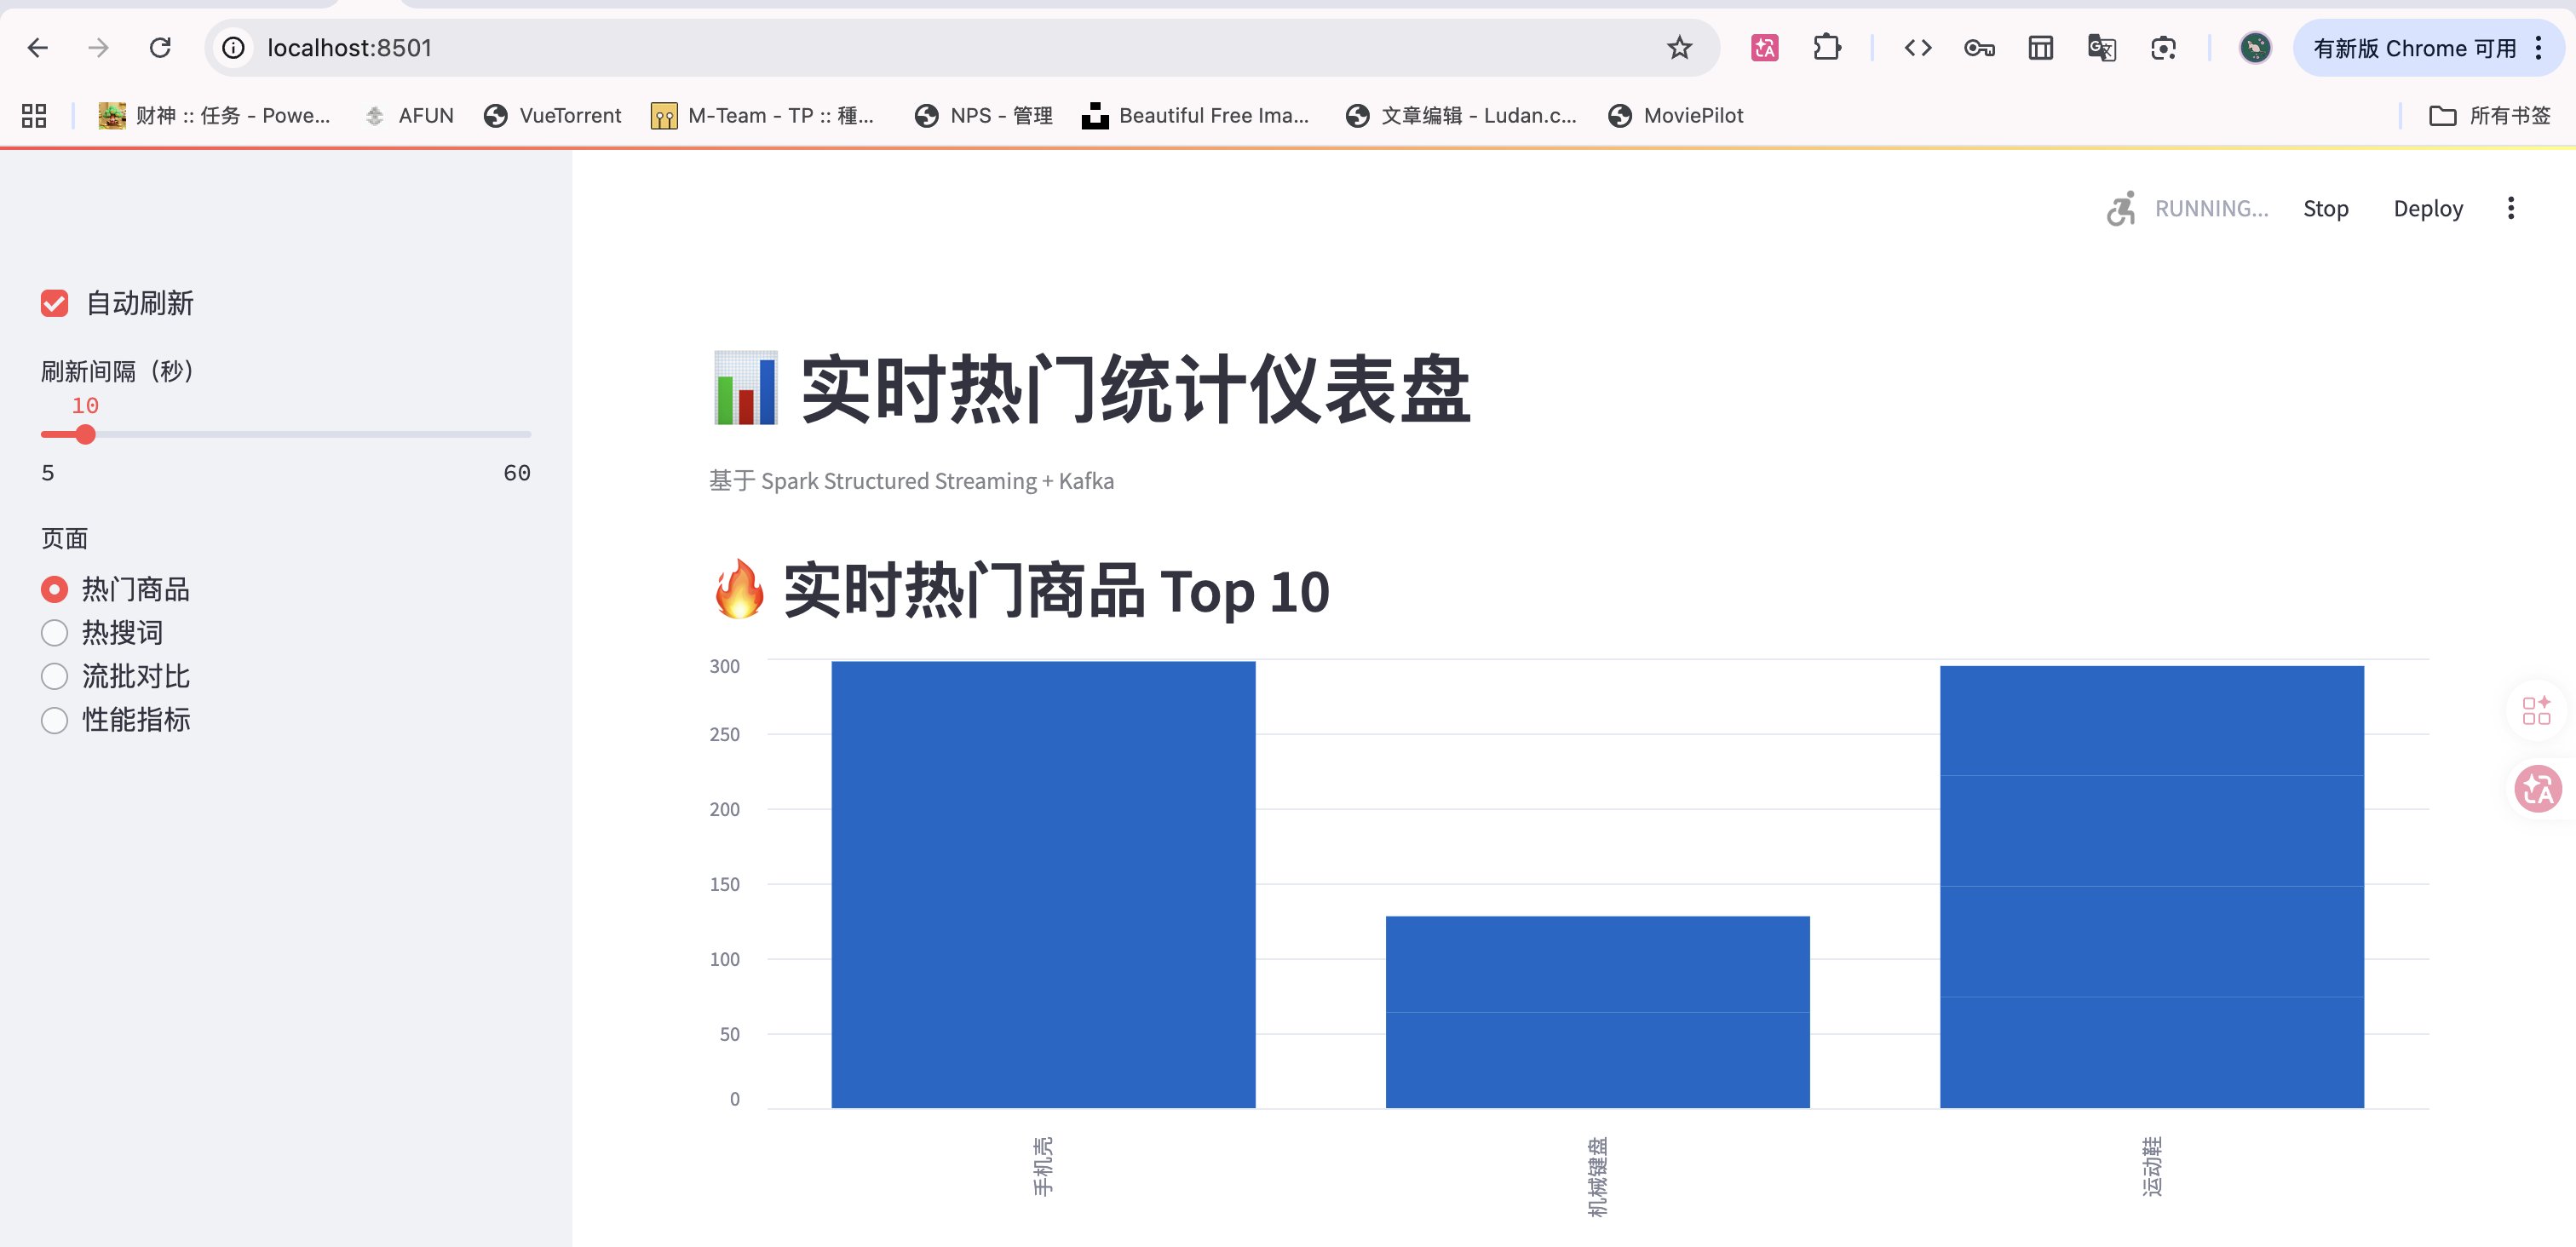
\includegraphics[width=0.95\textwidth]{figures/dashboard_hot_products.png}
\caption{Streamlit 仪表盘——实时热门商品 Top-10 柱状图}
\label{fig:dashboard-products}
\end{figure}

图~\ref{fig:dashboard-table} 展示了热门商品的详细数据表格，包含商品名称、分类和浏览次数，可以直观地看到手机壳（75次）、运动鞋（74次）、机械键盘（64次）位列前三。

\begin{figure}[H]
\centering
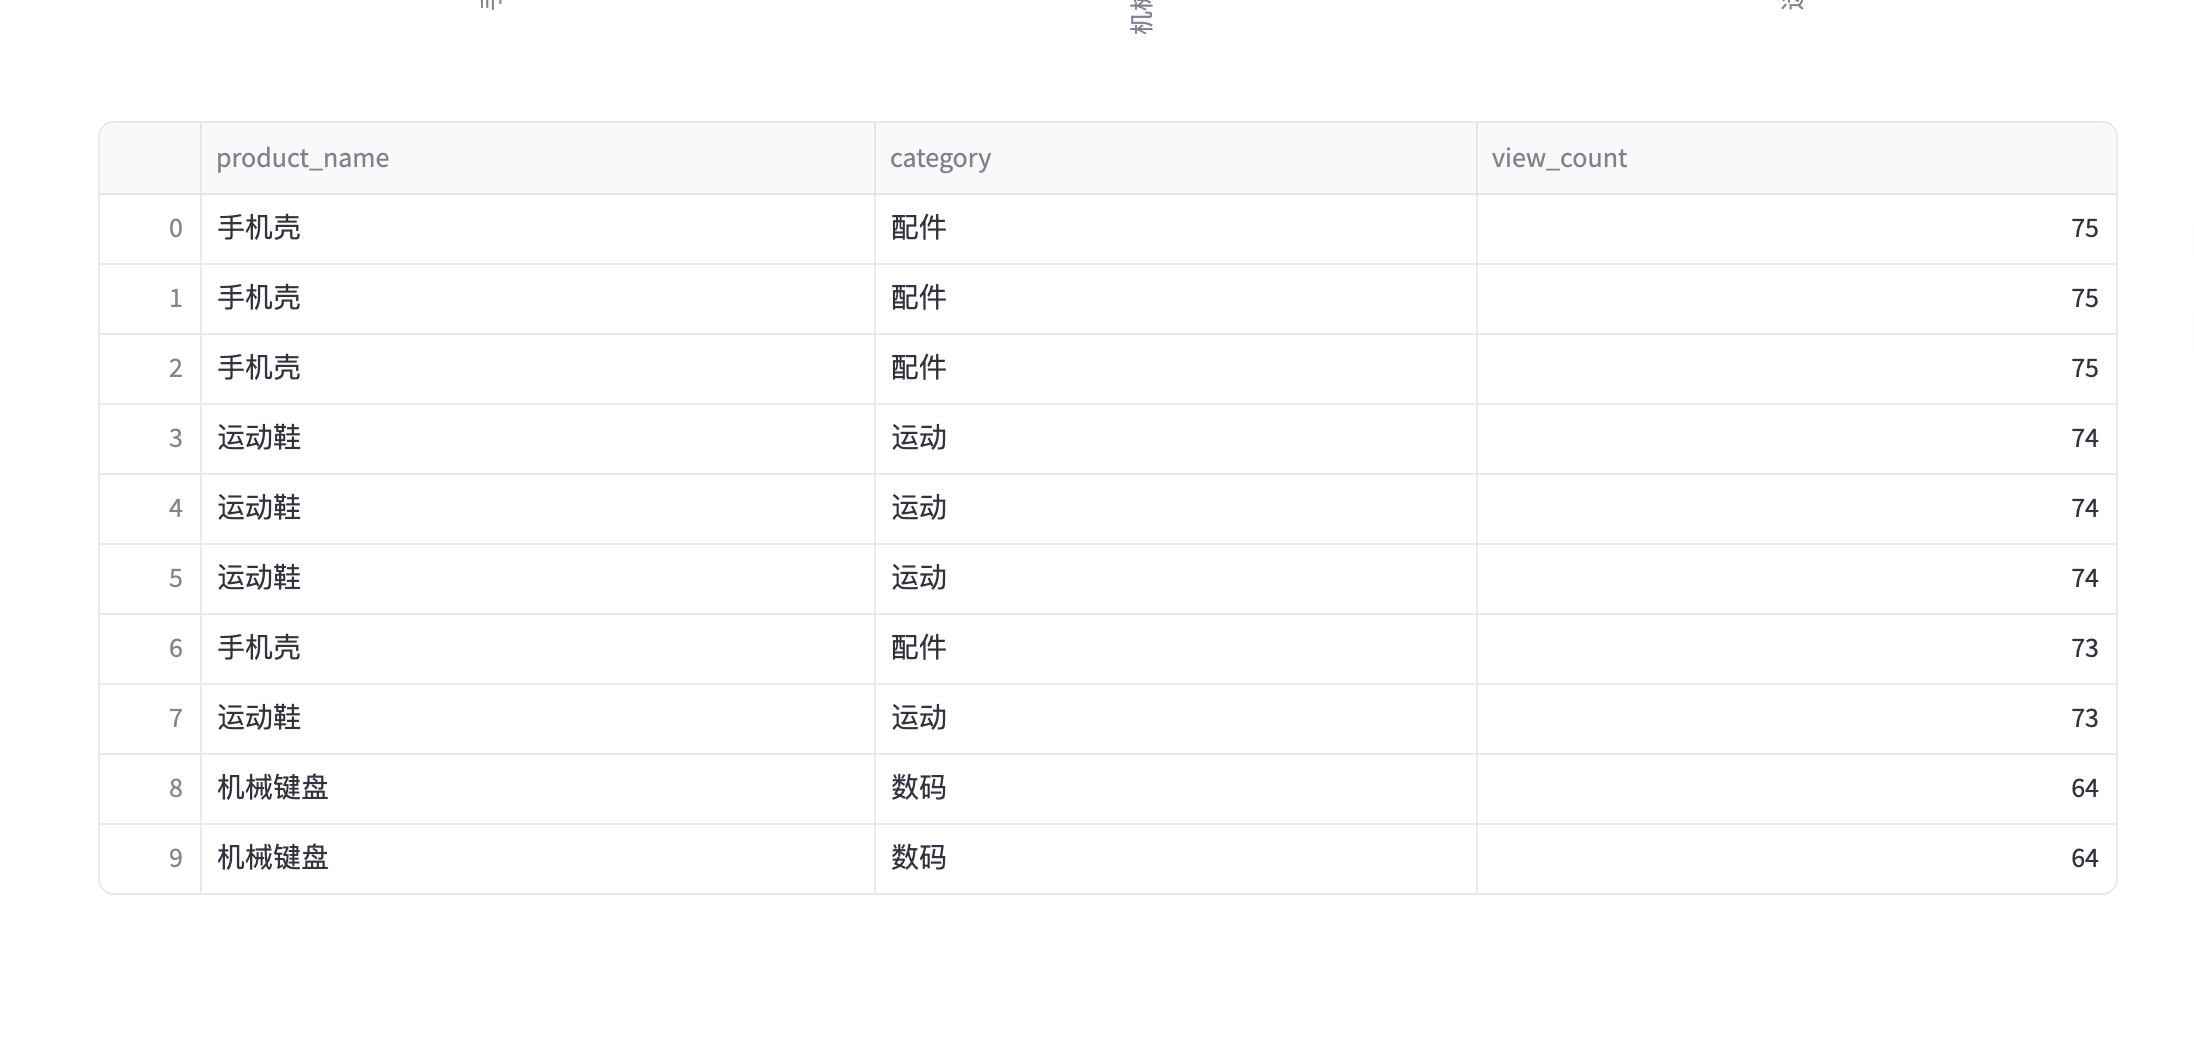
\includegraphics[width=0.95\textwidth]{figures/dashboard_table.png}
\caption{Streamlit 仪表盘——热门商品详细数据表}
\label{fig:dashboard-table}
\end{figure}

图~\ref{fig:dashboard-comparison} 展示了流处理与批处理的性能对比页面，左右两栏分别显示批处理（总记录数 50,000、总耗时 8.25s、吞吐量 6,063 条/秒）和流处理（微批次 10s、延迟 $\sim$10--15 秒）的核心指标。

\begin{figure}[H]
\centering
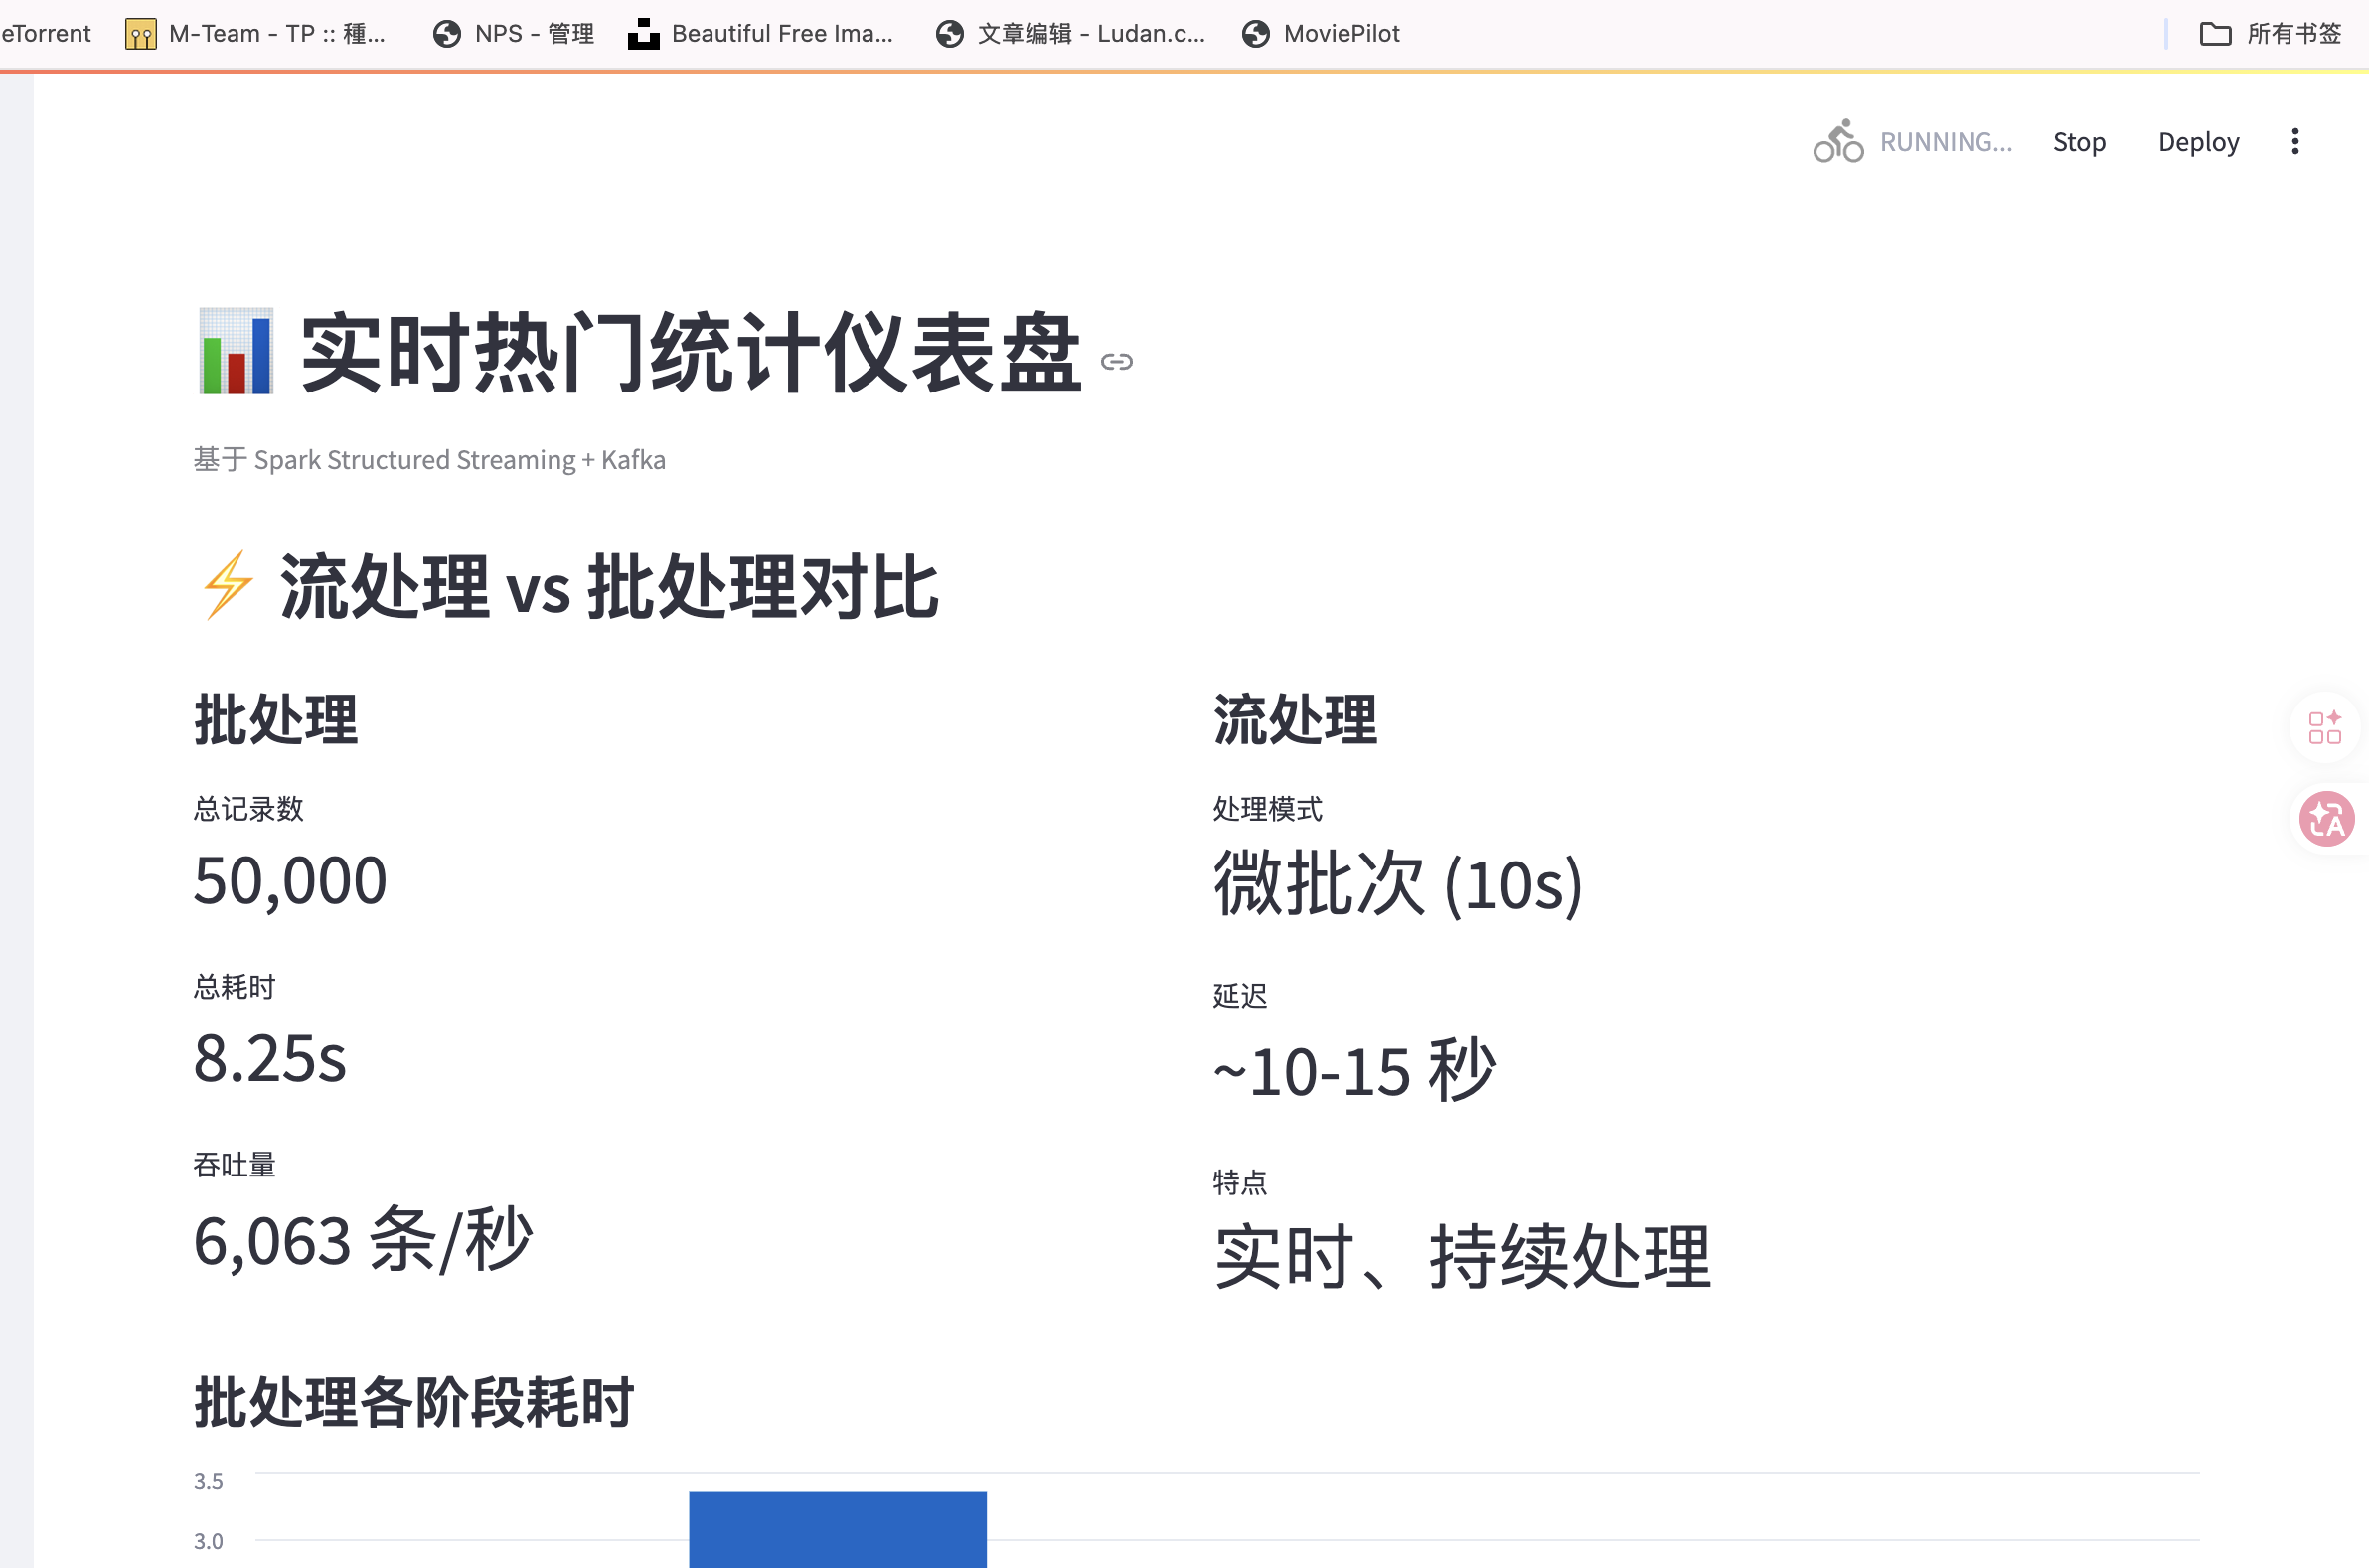
\includegraphics[width=0.95\textwidth]{figures/dashboard_comparison.png}
\caption{Streamlit 仪表盘——流处理 vs 批处理性能对比}
\label{fig:dashboard-comparison}
\end{figure}

% =================================================================
\section{总结与展望}
% =================================================================

\subsection{项目总结}

本项目成功构建了一个基于 Spark Structured Streaming + Kafka 的实时热门统计系统，主要成果包括：

\begin{enumerate}    \item 实现了热门商品 Top-10 和热搜词 Top-10 的\textbf{实时统计}，采用滑动窗口和 Watermark 处理乱序数据。
    \item 完成了流处理与批处理的\textbf{定量对比}，批处理吞吐量达 6,063 条/秒，流处理首条结果延迟 $\sim$10 秒。
    \item 通过 Docker 容器化实现了\textbf{一键部署}，降低了环境搭建的复杂度。
    \item 基于 Checkpoint 实现了\textbf{容错恢复}，保证了 Exactly-Once 语义。
    \item 通过 Streamlit 仪表盘实现了\textbf{实时可视化}，直观展示分析结果。
\end{enumerate}

\subsection{技术反思}

\begin{itemize}    \item \textbf{Watermark 阈值的选择}是一个 trade-off：阈值过小会丢弃合理的迟到数据，阈值过大会增加状态存储开销和结果延迟。
    \item \textbf{微批次 vs 连续处理}：本项目使用 Trigger 间隔为 10 秒的微批次模式。Spark 也支持 Continuous Processing 模式（毫秒级延迟），但目前仅支持有限的操作，不支持聚合。
    \item \textbf{JSON vs Parquet}：批处理的 40\% 时间花在数据加载上，改用 Parquet 格式可显著提升性能。
\end{itemize}

\subsection{未来展望}

\begin{enumerate}    \item \textbf{多节点集群}：将系统部署到多节点 Spark 集群，测试分布式环境下的可扩展性。
    \item \textbf{Exactly-Once 端到端验证}：通过注入故障和数据校验，严格验证端到端 Exactly-Once 语义。
    \item \textbf{实时告警}：在热门统计的基础上增加异常检测（如流量突增告警），扩展系统的实用价值。
    \item \textbf{生产级存储}：将结果写入 Redis 或时序数据库（如 InfluxDB），替代文件系统输出，支持高并发查询。
\end{enumerate}

% =================================================================
% 参考文献
% =================================================================
\begin{thebibliography}{99}
\bibitem{zaharia2016} Zaharia M, Xin R S, Wendell P, et al. Apache Spark: A Unified Engine for Big Data Processing[J]. Communications of the ACM, 2016, 59(11): 56-65.
\bibitem{armbrust2018} Armbrust M, Das T, Torres J, et al. Structured Streaming: A Declarative API for Real-Time Applications in Apache Spark[C]. Proceedings of the 2018 International Conference on Management of Data (SIGMOD), 2018: 601-613.
\bibitem{kreps2011} Kreps J, Narkhede N, Rao J. Kafka: A Distributed Messaging System for Log Processing[C]. Proceedings of the NetDB Workshop, 2011.
\bibitem{dean2004} Dean J, Ghemawat S. MapReduce: Simplified Data Processing on Large Clusters[C]. OSDI, 2004: 137-150.
\bibitem{spark-doc} Apache Spark Documentation: Structured Streaming Programming Guide. \url{https://spark.apache.org/docs/latest/structured-streaming-programming-guide.html}
\bibitem{kafka-doc} Apache Kafka Documentation. \url{https://kafka.apache.org/documentation/}
\end{thebibliography}

% =================================================================
% 附录
% =================================================================
\appendix
\section{团队分工}

\begin{table}[H]
\centering
\begin{tabular}{lp{10cm}}
\toprule
\textbf{成员} & \textbf{负责内容} \\
\midrule
赵英杰 (D23090600756) & 系统架构设计、Spark Streaming 核心开发、Kafka 环境搭建、性能测试 \\
韦多展 (D23090600792) & 数据生产者开发、批处理对比分析、可视化仪表盘、报告撰写 \\
\bottomrule
\end{tabular}
\end{table}

\section{项目代码结构}

\begin{lstlisting}[language=bash, caption={项目目录结构}]
realtime-hot-stats/
|-- docker-compose.yml          # Kafka Docker 编排
|-- Makefile                    # 常用命令封装
|-- requirements.txt            # Python 依赖
|-- data/
|   |-- products.json           # 50 个商品 (带权重)
|   |-- search_keywords.json    # 40 个搜索关键词 (带权重)
|-- src/
|   |-- producer/
|   |   |-- data_generator.py   # 加权随机数据生成
|   |   |-- kafka_producer.py   # Kafka 生产者
|   |-- streaming/
|   |   |-- common.py           # SparkSession + Schema
|   |   |-- hot_products.py     # 热门商品流处理
|   |   |-- hot_keywords.py     # 热搜词流处理
|   |-- batch/
|   |   |-- batch_analysis.py   # 批处理对比
|   |-- visualization/
|   |   |-- dashboard.py        # Streamlit 仪表盘
|   |-- benchmark/
|       |-- perf_test.py        # 性能测量
|-- output/                     # 运行结果输出
|-- notebooks/
    |-- analysis.ipynb          # 性能分析 Notebook
\end{lstlisting}

\end{document}
